% Created 2021-04-22 Thu 07:32
% Intended LaTeX compiler: pdflatex
\documentclass[presentation]{beamer}
\usepackage[utf8]{inputenc}
\usepackage[T1]{fontenc}
\usepackage{graphicx}
\usepackage{grffile}
\usepackage{longtable}
\usepackage{wrapfig}
\usepackage{rotating}
\usepackage[normalem]{ulem}
\usepackage{amsmath}
\usepackage{textcomp}
\usepackage{amssymb}
\usepackage{capt-of}
\usepackage{hyperref}
\RequirePackage{fancyvrb}
\DefineVerbatimEnvironment{verbatim}{Verbatim}{fontsize=\scriptsize}
\usetheme{metropolis}
\usecolortheme{}
\usefonttheme{}
\useinnertheme{}
\useoutertheme{}
\author{Petru Rebeja, Marius Apetrii}
\date{22 Aprilie 2021}
\title{Tehnici Avansate de Programare}
\subtitle{Baze de date}
\institute[UAIC]{Facultatea de Matematică\\Universitatea Alexandru Ioan Cuza, Iași}
\hypersetup{
 pdfauthor={Petru Rebeja, Marius Apetrii},
 pdftitle={Tehnici Avansate de Programare},
 pdfkeywords={},
 pdfsubject={},
 pdfcreator={Emacs 26.3 (Org mode 9.4.5)},
 pdflang={Romanian}}
\begin{document}

\maketitle
\section{Introducere}
\label{sec:orgbe95f49}
\begin{frame}[label={sec:org5dfeac3}]{Recapitulare}
\begin{itemize}
\item \alert{Test-Driven Development} --- un stil de dezvoltare software în care mai întâi se scriu testele pentru un anumit aspect iar mai apoi implementarea propriu-zisă.
\end{itemize}
\end{frame}
\begin{frame}[label={sec:orga875c79}]{Agenda}
\begin{itemize}
\item Baze de date
\item Istoricul schemei bazei de date relaționale
\item Proiectarea bazelor de date
\end{itemize}
\end{frame}
\section{Baze de date}
\label{sec:orgfb15d00}
\begin{frame}[label={sec:org0266291},fragile]{Noțiuni de bază}
 \begin{block}{Bază de date}
\vskip 0.1in
O \texttt{bază de date} este o colecție organizată de date care sunt stocate și accesate de pe un calculator\footnote{\url{https://en.wikipedia.org/wiki/Database}}.
\end{block}
\end{frame}
\begin{frame}[label={sec:org92ddfb8}]{Noțiuni de bază}
\begin{block}{Sistem de Gestiune al Bazelor de Date}
\vskip 0.1in
Sistemul de Gestiune a Bazelor de Date este un sistem software care le permite utilizatorilor să definească, să creeze, să întrețină și să controleze accesul la baza de date\footnote{Connolly, Thomas M.; Begg, Carolyn E. (2014). Database Systems – A Practical Approach to Design Implementation and Management (6th ed.). Pearson. p. 64. ISBN 978-1292061184.}.
\end{block}
\end{frame}
\begin{frame}[label={sec:orga3207eb}]{Noțiuni de bază}
\begin{block}{Schema bazei de date}
\vskip 0.1in
Schema bazei de date este structura logică a bazei de date descrisă într-un limbaj formal suportat de SGBD\footnote{\url{http://en.wikipedia.org/wiki/Database\_schema}} sau o reprezentare vizuală a acesteia\footnote{\url{https://www.techopedia.com/definition/30601/database-schema}}
\end{block}
\end{frame}
\begin{frame}[label={sec:orga38db46},fragile]{Tipuri de baze de date}
 Există două tipuri de baze de date:
\begin{itemize}
\item Relaționale (\texttt{SQL}) și
\item Non-relaționale (\texttt{No-SQL})
\end{itemize}
\end{frame}
\begin{frame}[label={sec:orgc7266b9}]{Baze de date relaționale}
\begin{itemize}
\item Sunt bazate pe tabele și modelează relația dintre ele,
\item Au o schemă predefinită,
\item Suportă interogări complexe,
\end{itemize}
\end{frame}
\begin{frame}[label={sec:org2ee4677},fragile]{Baze de date relaționale (cont.)}
 \begin{itemize}
\item Suportă creșterea pe verticală (\texttt{vertical scaling}) prin adăugarea de memorie RAM, spațiu pe disk etc.,
\item Pun accentul pe proprietățile \texttt{ACID}:
\begin{itemize}
\item \texttt{Atomicity} --- modificări atomice,
\item \texttt{Consistency} --- impune consistența datelor
\item \texttt{Isolation} --- modificările se fac în izolare unele față de altele
\item \texttt{Durability} --- modificările sunt salvate pe disk.
\end{itemize}
\end{itemize}
\end{frame}
\begin{frame}[label={sec:orgc446632}]{Baze de date No-SQL}
\begin{itemize}
\item Sunt bazate pe documente, grafuri, perechi cheie-valoare etc.
\item \alert{Nu} au o schemă predefinită,
\item Au suport limitat pentru interogări complexe,
\end{itemize}
\end{frame}
\begin{frame}[label={sec:orgc840f59},fragile]{Baze de date No-SQL (cont.)}
 \begin{itemize}
\item Suportă creșterea pe orizontală (\texttt{horizontal scaling}) prin adăugarea de noduri noi,
\item Aplică teorema CAP\footnote{\url{https://en.wikipedia.org/wiki/CAP\_theorem}} --- în orice moment oferă două proprietăți din următoarele:
\begin{itemize}
\item \texttt{Consistency} --- orice scriere primește cele mai recente date sau o eroare,
\item \texttt{Availability} --- fiecare cerere primește un răspuns dar datele pot să nu fie cele mai recente,
\item \texttt{Partition tolerance} --- systemul continuă să funcționeze în ciuda pierderii unor mesaje.
\end{itemize}
\end{itemize}
\end{frame}
\section{Evoluția bazei de date}
\label{sec:orgb369eb8}
\begin{frame}[label={sec:org4894448}]{Evoluția aplicației}
\begin{itemize}
\item Baza de date evoluează (de obicei) împreună cu aplicația,
\item Modificările bazei de date fac parte din ciclul de dezvoltare.
\end{itemize}
\end{frame}
\begin{frame}[label={sec:org38fd652}]{Bune practici}
\begin{itemize}
\item Schema bazei de date trebuie păstrată în sistemul de management al istoricului\footnote{\url{https://www.troyhunt.com/10-commandments-of-good-source-control/}} pentru a asigura sincronizarea între modificările aplicației și a bazei de date,
\item Aplicarea modificărilor trebuie sincronizată,
\item Altfel întregul sistem software devine inutilizabil.
\end{itemize}
\end{frame}
\section{Proiectarea bazelor de date}
\label{sec:orgf0b5ba6}
\begin{frame}[label={sec:orga8b0433},fragile]{Primary/Foreign Key}
 \begin{itemize}
\item O cheie primară (\texttt{Primary Key}) este o mulţime de coloane ale unui tabel a căror valori identifică în mod unic o înregistrare\footnote{\url{http://www.differencebetween.net/technology/difference-between-primary-key-and-unique-key/}}.
\item O cheie străină (\texttt{Foreign Key}) este o mulţime de coloane ale unui tabel care fac referinţă la o cheie primară\footnote{\url{https://www.w3schools.com/sql/sql\_foreignkey.asp}}.
\end{itemize}
\end{frame}
\begin{frame}[label={sec:org341f01c},fragile]{Relaţie}
 Adăugarea unei chei străine crează o \texttt{relaţie} între cele două tabele unde:
\begin{itemize}
\item Tabelul \texttt{copil} este cel care conţine cheia străină,
\item Tabelul \texttt{părinte} este cel care conţine cheia primară referenţiată de tabelul copil.
\end{itemize}
\end{frame}
\begin{frame}[label={sec:org2e0e1f2}]{Exemplu: 1*N}
\begin{center}
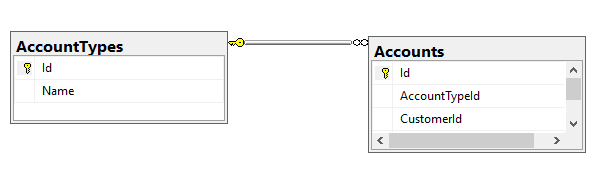
\includegraphics[width=\textwidth]{img/one-to-many.png}
\end{center}
\end{frame}
\begin{frame}[label={sec:orgcb471b1}]{Exemplu\footnote{\url{https://smehrozalam.wordpress.com/2010/06/29/entity-framework-queries-involving-many-to-many-relationship-tables}}: N*M}
\begin{center}
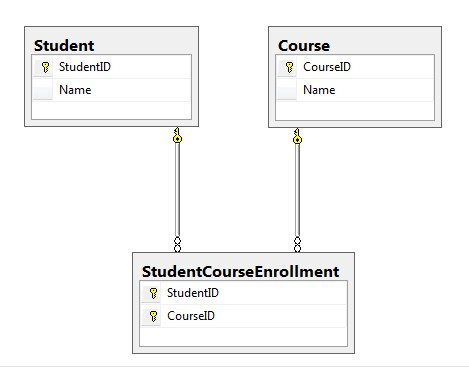
\includegraphics[width=.8\textwidth]{img/many-to-many.png}
\end{center}
\end{frame}
\begin{frame}[label={sec:orgd5a24d7}]{Normalizare}
\begin{block}{Normalizarea bazei de date}
\vskip 0.1in
Procesul de structurare a unei baze de date relaţionale pentru a reduce redundanţa datelor şi a îmbunătăţi integritatea acestora\footnote{\url{https://en.wikipedia.org/wiki/Database\_normalization}}.
\end{block}
\end{frame}
\begin{frame}[label={sec:org3faea94}]{Objectivele normalizării}
\begin{itemize}
\item Modelarea conceptelor din lumea reală şi a relaţiilor dintre acestea.
\item Extensibilitate sporită: adăugarea obiectelor noi se face cu intervenţie minimă.
\end{itemize}
\end{frame}
\begin{frame}[label={sec:org261f74e},fragile]{Forme normale}
 \begin{itemize}
\item Normalizarea se face prin aducerea schemei la o \texttt{formă normală}.
\item O \texttt{formă normală} este o proprietate a structurii bazei de date.
\item Există mai multe forme normale (\texttt{FN1}---\texttt{FN6} etc.).
\item O bază de date este normalizată dacă respectă cel puţin \texttt{FN3}.
\end{itemize}
\end{frame}
\begin{frame}[label={sec:orga2cce32},fragile]{Forma Normală 1}
 \begin{block}{FN1}
\vskip 0.1in
O relaţie este în \texttt{Forma Normală 1} dacă în fiecare coloană a unui tabel avem doar valori atomice.
\end{block}
\end{frame}
\begin{frame}[label={sec:org7680abf},fragile]{Forma Normală 1}
 Normalizarea la \texttt{FN1} se face prin:
\begin{enumerate}
\item Eliminarea grupurilor care se repetă.
\item Crearea unui table pentru fiecare colecţie de date cu coeziune mare.
\item Adăugarea unei chei primare.
\end{enumerate}
\end{frame}
\begin{frame}[label={sec:orgd298a16},fragile]{Forma Normală 2}
 \begin{block}{FN2}
\vskip 0.1in
O relaţie este în \texttt{Forma Normală 2} dacă:
\begin{enumerate}
\item Este în \texttt{Forma Normală 1} şi
\item Toate atributele unui tabel depind doar de cheia primară direct sau indirect.
\end{enumerate}
\end{block}
\end{frame}
\begin{frame}[label={sec:org04fc742}]{Forma Normală 2}
Tournament winners\footnote{\url{https://en.wikipedia.org/wiki/Third\_normal\_form}}
\begin{center}
\begin{tabular}{lrll}
\uline{Tournament} & \uline{Year} & Winner & Winner's date of birth\\
\hline
Indiana Invitational & 1998 & Al Fredrickson & 21 July 1975\\
Cleveland Open & 1999 & Bob Albertson & 28 September 1968\\
Des Moines Masters & 1999 & Al Fredrickson & 21 July 1975\\
Indiana Invitational & 1999 & Chip Masterson & 14 March 1977\\
\end{tabular}
\end{center}
\end{frame}
\begin{frame}[label={sec:orgd2d505d},fragile]{Forma Normală 3}
 \begin{block}{FN3}
\vskip 0.1in
O relaţie este în \texttt{Forma Normală 3} dacă:
\begin{enumerate}
\item Este în \texttt{Forma Normală 2} şi
\item Fiecare atribut depinde direct de cheia primară.
\end{enumerate}
\end{block}
\end{frame}
\begin{frame}[label={sec:orge908731}]{Forma Normală 3\footnote{\url{https://en.wikipedia.org/wiki/Third\_normal\_form}}}
\begin{center}
\begin{tabular}{lrl}
Tournament & Year & Winner\\
\hline
Indiana Invitational & 1998 & Al Fredrickson\\
Cleveland Open & 1999 & Bob Albertson\\
Des Moines Masters & 1999 & Al Fredrickson\\
Indiana Invitational & 1999 & Chip Masterson\\
\end{tabular}
\end{center}
\begin{center}
\begin{tabular}{ll}
Winner & Date of birth\\
\hline
Chip Masterson & 14 March 1977\\
Al Fredrickson & 21 July 1975\\
Bob Albertson & 28 September 1968\\
\end{tabular}
\end{center}
\end{frame}
\section{Încheiere}
\label{sec:org8989fe9}
\begin{frame}[label={sec:orgcb4a5f1},fragile]{Recapitulare --- baze de date}
 \begin{itemize}
\item \alert{Baza de date} este o colecție organizată de date care pot fi manipulate prin intermediul unui SGBD.
\item \alert{SGBD} = Sistem de Gestiune al Bazelor de Date; permite manipulearea datelor și întreținerea bazelor de date.
\item \alert{Schema bazei de date} este reprezentarea structurii bazei de date și trebuie păstrată în sistemul de gestiune al istoricului alături de codul-sursă al aplicației.
\item Folosiți \texttt{Database project} din Visual Studio pentru modificarea schemei bazei de date.
\end{itemize}
\end{frame}
\begin{frame}[label={sec:orgc939f9a},fragile]{Recapitulare --- ACID}
 \begin{itemize}
\item \texttt{Atomicity} --- modificări atomice,
\item \texttt{Consistency} --- impune consistența datelor
\item \texttt{Isolation} --- modificările se fac în izolare unele față de altele
\item \texttt{Durability} --- modificările sunt salvate pe disk.
\end{itemize}
\end{frame}
\begin{frame}[label={sec:org9bf4e97},fragile]{Recapitulare --- proiectarea bazei de date}
 \begin{itemize}
\item Elemente esenţiale în proiectarea bazelor de date: \texttt{cheie primară}, \texttt{cheie străină} şi \texttt{relaţie}.
\item \texttt{Normalizare} --- proiectarea/restructurarea bazei de date pentru a o aduce în (cel puţin) \texttt{forma normală 3}.
\item O schemă este în \texttt{forma normală 3} (\texttt{FN3}) dacă atributele fiecărui tabel sunt atomice și depind doar de cheia primară.
\end{itemize}
\end{frame}
\begin{frame}[label={sec:orgb25f1fa}]{Vă mulțumesc}
\begin{center}
Mulțumesc pentru atenție!
\end{center}
\end{frame}
\end{document}